\documentclass[9pt,aspectratio=43]{beamer}
\usepackage{tikz}
\usetheme{default}
\setbeamertemplate{navigation symbols}{}
\title{Incremental analysis: experiments and bounds}
\subtitle{Generated interaction study}
\author{Research group}
\date{}
\year=2026\month=11\day=5
\newcommand{\fuzzlayerA}[1]{\textit{#1}}
\newcommand{\fuzzlayerB}[1]{\fuzzlayerA{#1}}
\newcommand{\fuzzlayerC}[1]{\fuzzlayerB{#1}}
\newcommand{\fuzzterm}[1]{\fuzzlayerC{#1}}
\newcommand{\fuzzpair}[2]{\fuzzterm{#1}: #2}
\newcommand{\fuzzunit}{ms}
\let\fuzzoriginalunit\fuzzunit
\newcommand{\fuzzcoefficient}{1}
\newcommand{\fuzzscale}[2][\fuzzcoefficient]{#1\,#2}
\definecolor{fuzzpaint}{RGB}{255,0,255}
\definecolor{fuzzsecond}{RGB}{18,137,67}
\tikzset{fuzzvertex/.style={draw,rounded corners=1pt,fill=blue!10,inner sep=1pt,minimum width=.35cm,minimum height=.25cm}}
\begin{document}
\section{Incremental analysis}
\begin{frame}[t,shrink=5]{Incremental analysis}{Composed dependencies}
\fuzzpair{Experiment}{Timing: 12\fuzzunit; estimate $\fuzzscale{x}+\fuzzscale[2]{y}$.}\par
{\renewcommand{\fuzzunit}{cycles}\let\fuzzterm\textbf\fuzzpair{LocalScope}{Timing: 7\fuzzunit.}\par}
\fuzzpair{RestoredScope}{Timing: 11\fuzzunit.}\par
\begin{columns}[onlytextwidth,t]
\begin{column}{0.38\textwidth}
\begin{flushleft}
\begin{tabular}{lrr}Method&Cost&Error\\\hline
Cached0&25&21\\
Global1&26&8\\
Global2&18&27\\
Global3&13&7\\
\end{tabular}
\end{flushleft}
\par
\[E=\sum_{i=1}^{n}w_i x_i\]
\par
\begin{tabular}{lrr}Method&Cost&Error\\\hline
Local0&27&8\\
Global1&28&21\\
Global2&28&10\\
Fresh3&15&29\\
\end{tabular}
\par
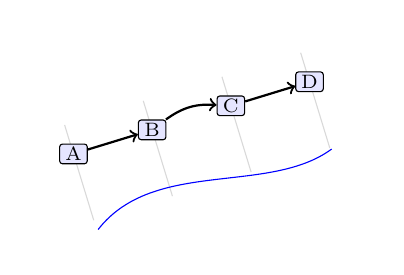
\begin{tikzpicture}[font=\scriptsize]
\begin{scope}[scale=1.1,rotate=17]
\clip (-.4,-1) rectangle (3.350,.5);
\foreach \x in {0,1,2,3} {\draw[gray!30] (\x*0.950,-.8)--(\x*0.950,.35);}
\node[fuzzvertex] (g7n0) at (0.000,0) {A};
\node[fuzzvertex] (g7n1) at (0.950,0) {B};
\node[fuzzvertex] (g7n2) at (1.900,0) {C};
\node[fuzzvertex] (g7n3) at (2.850,0) {D};
\begin{scope}[xshift=.5pt,yshift=-.5pt]
\draw<2->[->,thick] (g7n0) -- (g7n1);
\draw<2->[->,thick] (g7n1) to[bend left=20] (g7n2);
\draw<2->[->,thick] (g7n2) -- (g7n3);
\draw[blue] (0,-.9) .. controls (0.855,-.3) and (1.995,-1.1) .. (2.850,-.8);
\end{scope}
\end{scope}
\end{tikzpicture}
\par
\begin{itemize}
\item \[E=\sum_{i=1}^{n}w_i x_i\]
\item \textit{Intermediate results carry} both a numerical estimate and an explicit dependency set.  The estimate is $x_i+x_{i+1}$.
\end{itemize}
\end{column}
\begin{column}{0.58\textwidth}
\begin{enumerate}
\item \begin{flushright}
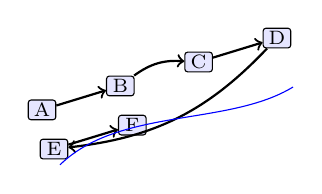
\begin{tikzpicture}[font=\scriptsize]
\begin{scope}[scale=0.8,rotate=17]


\node[fuzzvertex] (g13n0) at (0.000,0) {A};
\node[fuzzvertex] (g13n1) at (1.300,0) {B};
\node[fuzzvertex] (g13n2) at (2.600,0) {C};
\node[fuzzvertex] (g13n3) at (3.900,0) {D};
\node[fuzzvertex] (g13n4) at (0.000,-0.65) {E};
\node[fuzzvertex] (g13n5) at (1.300,-0.65) {F};
\begin{scope}[xshift=.5pt,yshift=-.5pt]
\draw<1->[->,thick] (g13n0) -- (g13n1);
\draw<1->[->,thick] (g13n1) to[bend left=20] (g13n2);
\draw<1->[->,thick] (g13n2) -- (g13n3);
\draw<1->[->,thick] (g13n3) to[bend left=20] (g13n4);
\draw<1->[->,thick] (g13n4) -- (g13n5);
\draw[blue] (0,-.9) .. controls (1.170,-.3) and (2.730,-1.1) .. (3.900,-.8);
\end{scope}
\end{scope}
\end{tikzpicture}
\end{flushright}
\item \begin{description}
\item[Stage 1] \[\begin{aligned}a+b&=c\\ d-e&=f\end{aligned}\]
\item[Stage 2] \textrm{A local update} can change the measurements used by several neighboring components.  The estimate is $\frac{a+b}{1+c}$.
\end{description}
\item \begin{flushright}
\[E=\sum_{i=1}^{n}w_i x_i\]
\end{flushright}
\end{enumerate}
\end{column}
\end{columns}
\par 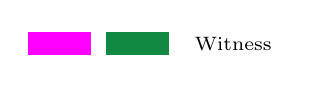
\begin{tikzpicture}[font=\scriptsize]
\fill<2-3>[fuzzpaint] (0,0) rectangle (.8,.3);
\fill<3->[fuzzsecond] (1,0) rectangle (1.8,.3);
\node[anchor=west] at (2,0.15) {Witness};
\end{tikzpicture}
\only<4>{}
\end{frame}
\renewcommand{\fuzzunit}{steps}
\renewcommand{\fuzzcoefficient}{2}
\renewcommand{\fuzzterm}[1]{{\textbf{#1}}}
\section{Constraint propagation}
\begin{frame}[t]{Constraint propagation}
\fuzzpair{MacroStageB}{Timing: 12\fuzzunit, retained: 9\fuzzoriginalunit.}\par
{\renewcommand{\fuzzunit}{local}\fuzzpair{FrameLocal}{Timing: 5\fuzzunit.}\par}
\fuzzpair{FrameRestored}{Timing: 8\fuzzunit; estimate $\fuzzscale{x}$.}\par
\begin{columns}[T]\begin{column}{.46\textwidth}We compare the proposed solution with a reference computed from the complete input.\end{column}\begin{column}{.46\textwidth}\begin{itemize}\item Input state\item Updated state\end{itemize}\end{column}\end{columns}
\end{frame}
\renewcommand{\fuzzunit}{Hz}
\renewcommand{\fuzzcoefficient}{3}
\renewcommand{\fuzzterm}[1]{{\textrm{#1}}}
\section{Iterative refinement}
\begin{frame}[t]{Message passing}
\fuzzpair{MacroStageC}{Timing: 12\fuzzunit, retained: 9\fuzzoriginalunit.}\par
{\renewcommand{\fuzzunit}{local}\fuzzpair{FrameLocal}{Timing: 5\fuzzunit.}\par}
\fuzzpair{FrameRestored}{Timing: 8\fuzzunit; estimate $\fuzzscale{x}$.}\par
\begin{block}{Follow-up}\fuzzterm{A revised value} depends on the preceding frame.\end{block}
\[r_{k+1}=r_k-\alpha d_k\]
\end{frame}
\renewcommand{\fuzzunit}{us}
\renewcommand{\fuzzcoefficient}{4}
\renewcommand{\fuzzterm}[1]{{\textrm{#1}}}
\section{Incremental analysis}
\begin{frame}[t]{Iterative refinement}
\fuzzpair{MacroStageD}{Timing: 12\fuzzunit, retained: 9\fuzzoriginalunit.}\par
{\renewcommand{\fuzzunit}{local}\fuzzpair{FrameLocal}{Timing: 5\fuzzunit.}\par}
\fuzzpair{FrameRestored}{Timing: 8\fuzzunit; estimate $\fuzzscale{x}$.}\par
\begin{columns}[T]\begin{column}{.46\textwidth}A local update can change the measurements used by several neighboring components.\end{column}\begin{column}{.46\textwidth}\begin{itemize}\item Input state\item Updated state\end{itemize}\end{column}\end{columns}
\end{frame}
\end{document}
